\documentclass{mulcia_aa}

\name{Nombre}
\lastName{Apellidos}

\begin{document}
\genTitle
\genAdvice

\begin{question}
¿Cuántas posibles hipótesis podemos representar mediante árboles de decisión si tenemos $n$ atributos binarios?
\end{question}
\begin{solution}
Solución
\end{solution}

\begin{question}
Definimos el tamaño de un árbol como el número de sus nodos, incluida las hojas. Dar dos árboles de tamaño distinto que representen la misma hipótesis.
\end{question}
\begin{solution}
Solución
\end{solution}

\begin{question}
Dado el conjunto de entrenamiento
\vspace{-10pt}
\begin{table}[!htbp]
\begin{align*}
    \begin{tabular}{|lllllll|}
    \hline
    Cielo   & Temperatura & Humedad & Viento & Agua     & Previsión & Deporte \\ \hline
    Soleado & Templada    & Normal  & Fuerte & Templada & Igual     & Sí      \\
    Soleado & Templada    & Alta    & Fuerte & Templada & Igual     & Sí      \\
    Lluvia  & Fría        & Alta    & Fuerte & Templada & Cambio    & No      \\
    Soleado & Templada    & Alta    & Fuerte & Fría     & Cambio    & Sí      \\ \hline
    \end{tabular}
\end{align*}
\end{table}
\vspace{-20pt}
\begin{flushleft}
y como conjunto de hipótesis $\mathcal{H}$ el conjunto de \emph{todos} los árboles de decisión, dar dos elementos del espacio de versiones $VS$. Uno de ellos debe clasificar de manera positiva y otro de manera negativa el ejemplo
\end{flushleft}

\centering$\langle Lluvia, Templada, Normal, Fuerte, Templada, Cambio \rangle$
\end{question}
\begin{solution}
Solución
\end{solution}
 
\begin{question}
En un problema de aprendizaje sobre el que vamos a aplicar el algoritmo ID3 se considera un conjunto de entrenamiento $D$ con $N$ ejemplos. Supongamos que hay un atributo $Atr_1$ que puede tomar $N$ valores y que cada uno de los ejemplos de $D$ toma en $Atr_1$ un valor distinto. Calcular \emph{Ganancia}($D$, $Atr_1$).
\end{question}
\begin{solution}
Solución
\end{solution}

\begin{question}
Demostrar que si $D$ es un conjunto de entrenamiento para un concepto $C$ entonces el algoritmo ID3 devuelve una hipótesis consistente con $D$ cualquiera que sea el criterio para elegir el \emph{mejor} atributo.
\end{question}
\begin{solution}
Solución
\end{solution}

\begin{question}
Sea $U$ un universo finito y sea $C$ un concepto sobre $U$ donde las instancias se representan como $n$-uplas de pares atributo-valor. Entonces $C$ puede representarse como un árbol de decisión.
\end{question}
\begin{solution}
Solución
\end{solution}

\begin{question}
Responder razonadamente si las siguientes afirmaciones son verdaderas o falsas. Si la respuesta \textbf{Verdadera} debes dar razones que apoyen tu decisión. Si la respuesta es \textbf{Falsa} debes dar un ejemplo en el que no se verifique la afirmación.
\end{question}
\begin{solution}
    \begin{enumerate}[label=(\alph*)]
        \item Sea $D_1 = \{e1,..., en\}$ un conjunto de entrenamiento y sea $D_2$ el conjunto de entrenamiento formado a partir de $D_1$ donde cada ejemplo se considera dos veces, esto es, $D_2 = \{e_1,...,e_n,e_{n+1},...,e_{2n}\}$ donde $\forall i\in\{1,...,n\}e_i = e_{i+n}$. Afirmación: \emph{El árbol de decisión obtenido mediante el algoritmo ID3 a partir de $D_1$ y $D_2$ son el mismo}.\\
        
        Solución    
        
        \item Tenemos un conjunto con $4n$ ejemplos y lo dividimos en dos partes: un conjunto de entrenamiento con $3n$ ejemplos y un conjunto de prueba con $n$ ejemplos. En el conjunto de entrenamiento $2n$ ejemplos son positivos y $n$ ejemplos son negativos. En el conjunto de prueba, los $n$ ejemplos que hay son todos positivos. Construimos el árbol de decisión A a partir del conjunto de entrenamiento mediante el algoritmo ID3. Afirmación: \emph{El árbol A contiene al menos un nodo tal que si podamos en ese nodo mejoramos el rendimiento respecto al conjunto de prueba.}\\
        
        Solución    
        
        \item Sean $D_1$ y $D_2$ dos conjuntos de entrenamiento para el mismo concepto. Entonces
        
        \begin{align}
            \frac{Ent(D_1)+Ent(D_2)}{2}\le Ent(D_1\cup D_2)
        \end{align}

        
        Solución
        
        \item Sean $D_1$ y $D_2$ dos conjuntos de entrenamiento para el mismo concepto tales que $D_1 \cap D_2 \not = \emptyset$. Entonces $Ent(D_1 \cup D_2) < Ent(D_1) + Ent(D_2)$.\\

        Solución
    \end{enumerate}
\end{solution}

\begin{question}
La ganancia de información en el algoritmo ID3 sólo sirve para hacer árboles más pequeños. Si aplicamos el algoritmo de árboles de decisión sobre un mismo conjunto de entrenamiento dos veces, la primera utilizando la ganacia de información para elegir el mejor atributo y la segunda vez utilizando otro criterio, entonces los dos árboles obtenidos pueden tener distinto tamaño, pero representan la misma hipótesis. \textbf{¿Verdadero o falso?}
\end{question}
\begin{solution}
Solución
\end{solution}

\begin{problem}
Supongamos que hemos dividido un conjunto de 25 ejemplos en dos conjuntos. El primero $D$ con 20 ejemplos lo hemos usado para crear un árbol de decisión y el segundo \emph{Prueba}, con 5 ejemplos, los vamos a usar para aplicar el \textsc{Algoritmo de poda para reducir el error}. El árbol obtenido y el conjunto de prueba son los siguientes:\\

{\centering
\begin{minipage}{0.45\textwidth}
   \centering
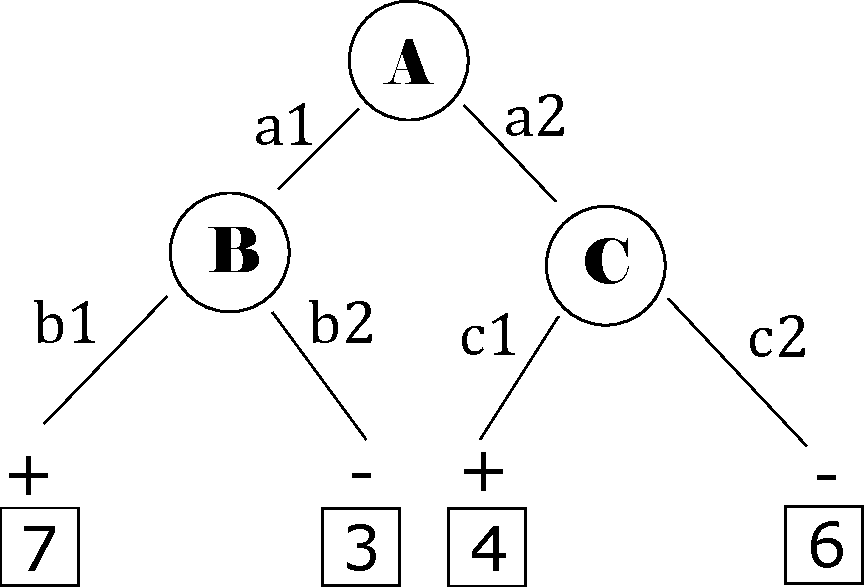
\includegraphics[width=60mm]{arbol-c3.pdf}
\end{minipage}
\begin{minipage}{0.45\textwidth}
   \centering
\begin{tabular}{|c|c|c|c|c|}
\hline
\textit{} & \textbf{A} & B  & C  & Cl. \\ \hline
$e_1$      & a1         & b1 & c1 & +   \\ \hline
$e_2$      & a2         & b1 & c2 & +   \\ \hline
$e_3$      & a1         & b2 & c1 & +   \\ \hline
$e_4$      & a1         & b2 & c2 & +   \\ \hline
$e_5$      & a2         & b2 & c1 & +   \\ \hline
\end{tabular}
\end{minipage}
}

\begin{flushleft}
Junto a la clasificación de cada hoja aparece el número de elementos del conjunto $D$ que verifica la condición, esto es, hay 7 ejemplos con A=a1 y B=b1 que tienen clasificación $+$, hay 3 ejemplos con A=a1 y B=b2 que tienen clasificación $-$, etc. Se pide usar el \textsc{Algoritmo de poda para reducir el error} sobre el árbol usando el conjunto \emph{Prueba}. \textbf{Especificar claramente cuál es el árbol obtenido}.
\end{flushleft}
\end{problem}

\begin{solution}
Solución
\end{solution}

\noindent\hrulefill
\begin{problem}
\textbf{Ejercicio opcional:} Demostrar que la ganancia de información es siempre mayor o igual a cero.
\end{problem}
\begin{solution}
Solución
\end{solution}
\end{document}
